\documentclass[11pt]{article}

\usepackage{fontspec}
\setmainfont{TeX Gyre Pagella}
\usepackage{amsmath}
\usepackage{amssymb}
\usepackage{mathtools}
\usepackage{geometry}
\geometry{margin=1.2in}
\usepackage{titling}
\usepackage[hidelinks]{hyperref}
\usepackage{tikz}
\usepackage{float}
\usepackage{listings}
\usepackage{xcolor}

\lstdefinelanguage{Rust}{
  keywords={fn,let,mut,struct,enum,impl,match,if,else,for,in,return,use,pub,self,Self,true,false},
  keywordstyle=\bfseries,
  sensitive=true,
  comment=[l]{//},
  morecomment=[l]{///},
  string=[b]"
}
\lstset{
  language=Rust,
  basicstyle=\ttfamily\small,
  columns=fullflexible,
  breaklines=true,
  frame=single,
  showstringspaces=false,
  commentstyle=\itshape,
  numbers=left,
  numberstyle=\tiny,
  xleftmargin=1.5em
}
\usetikzlibrary{arrows.meta,positioning,fit,calc}

\title{\textbf{Structural Honesty: The Preservation of Recoverable Warrant Across Transformations}}
\author{Flyxion \\ \textit{Independent Researcher}}
\date{\today}

\begin{document}
\maketitle

\begin{abstract}
Structural honesty is the requirement that the apparent epistemic strength of a claim, representation, abstraction, or intervention not exceed the warrant supplied by its supporting structure. It is distinct from sincerity, from ordinary factual accuracy, and from epistemic humility considered as a personal virtue. Sincerity concerns the relationship between an agent's assertions and that agent's beliefs; factual accuracy concerns the relationship between a statement and the world; structural honesty concerns the relationship between the apparent strength of a representation and the strength actually licensed by the structure beneath it. A statement can be sincere and factually correct while nevertheless implying more than its evidence supports, simply by virtue of how it is presented, formalized, compressed, or embodied. This essay argues that a single prohibition recurs across an otherwise disparate set of theoretical commitments developed in the wider research program: conjecture must not be presented as theorem, local consistency must not be presented as global realizability, detection must not be presented as repair warrant, an endpoint must not be presented as equivalent to the trajectory that produced it, a compressed representation must not be presented as lossless, a synthetic artifact must not be presented as testifying to a history it never had, an artifact must not be presented as though its interpretive key were unnecessary, and executability must not be presented as permission. Each of these is an instance of a single logical form: a weaker relation must not be silently promoted into a stronger one without an independent bridge principle that licenses the promotion. The essay traces this prohibition from its most literal origin, the marking of a conjecture as a conjecture, through representation, locality, intervention, provenance, compression, material artifacts, and finally refusal, arriving at a definition considerably more precise than ``do not lie'': structural honesty is the preservation of recoverable warrant across transformations, together with a prohibition against fabricating warrant that never existed.
\end{abstract}

\newpage

\section{Epistemic Honesty Before Structural Honesty}

The place to begin is not with a new term but with an old and almost mundane habit. Throughout the mathematical and theoretical essays comprising this research program, claims have been deliberately marked according to their epistemic type: definitions are distinguished from propositions, propositions from theorems, theorems from conjectures, conjectures from ansätze, and formal derivations from phenomenological or empirical interpretation. At first glance this looks like ordinary scholarly housekeeping, the sort of thing any careful author does out of professional habit. The claim of this essay is that something considerably stronger is already implicit in the practice, and that everything which follows is simply this same practice generalized to progressively larger objects.

A conjecture does not become a theorem merely because it is surrounded by valid mathematics. A result derived from an ansatz does not thereby establish the ansatz; the derivation inherits the ansatz's epistemic status rather than upgrading it. A numerical observation that happens to agree with a proposed model does not become an analytic result simply because the agreement is striking. A property that has been stipulated by definition cannot later be presented as though it had been independently discovered. In each case, the danger is not falsehood in the ordinary sense. The danger is that a correct local operation, embedded in an otherwise rigorous structure, can quietly inherit a strength it was never separately shown to possess.

This yields the most primitive form of the principle under discussion:

\[
\boxed{\text{Presentation must preserve epistemic status.}}
\]

Everything that follows can be understood as an expansion of this rule outward from propositions to representations, from representations to interventions, from interventions to histories, and eventually from histories to physical artifacts. The term for the general failure mode, when a weaker epistemic status is transformed into a stronger apparent one without additional warrant, is epistemic laundering. Structural honesty is the discipline that prevents it.

\section{Unlicensed Promotion}
\label{sec:promotion}

The theorem/conjecture distinction is a single instance of a considerably more general structure, and making that structure explicit is the theoretical center of this essay. Let $R_{\mathrm{weak}}$ and $R_{\mathrm{strong}}$ denote two relations between objects, where $R_{\mathrm{strong}}$ implies a stronger form of equivalence, warrant, or entitlement than $R_{\mathrm{weak}}$. The recurring error across every framework considered below has the same shape:

\[
R_{\mathrm{weak}}(x,y) \not\Rightarrow R_{\mathrm{strong}}(x,y)
\]

unless some independent bridge principle establishes the implication. Plausibility does not imply truth. Local consistency does not imply global realizability. Detection of a discrepancy does not imply diagnosis of its cause, and diagnosis does not imply that a repair is warranted. Two states sharing a present configuration do not thereby share a history. A successful reconstruction does not imply that the compression which preceded it was lossless. Physical or computational possibility does not imply normative or semantic admissibility.

Two complementary failure modes deserve to be distinguished at the outset, because both recur throughout what follows and they are easy to conflate. The first is promotion: producing an output that implies more warrant than the input actually supports, as when a conjecture is written in a tone appropriate to an established result. The second is externalization: leaving an endpoint intact and apparently usable while removing from it the structure necessary to understand how it was generated, why it may be trusted, how it might be repaired, or how it could be reproduced. These initially look unrelated, one a matter of overstatement and the other a matter of omission. They will turn out to be dual failures. Promotion adds warrant that was never earned; externalization removes the structure by which warrant could, in principle, be independently recovered. Structural honesty must guard against both.

\begin{figure}[ht]
\centering
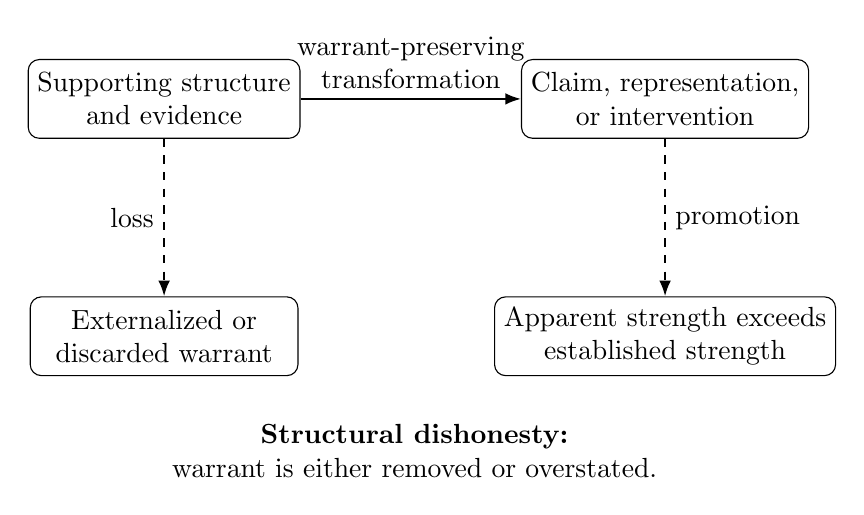
\begin{tikzpicture}[
    node distance=2.0cm and 2.8cm,
    box/.style={draw, rounded corners, align=center,
                minimum width=3.4cm, minimum height=1.0cm},
    arr/.style={-{Latex[length=2mm]}, thick}
]

\node[box] (structure) {Supporting structure\\and evidence};
\node[box, right=of structure] (claim) {Claim, representation,\\or intervention};

\draw[arr] (structure) -- node[above, align=center]
    {warrant-preserving\\transformation} (claim);

\node[box, below=of structure] (external)
    {Externalized or\\discarded warrant};
\node[box, below=of claim] (promotion)
    {Apparent strength exceeds\\established strength};

\draw[arr, dashed] (structure) -- node[left] {loss} (external);
\draw[arr, dashed] (claim) -- node[right] {promotion} (promotion);

\node[below=1.0cm of $(external)!0.5!(promotion)$, align=center]
    {\textbf{Structural dishonesty:}\\
     warrant is either removed or overstated.};

\end{tikzpicture}
\caption{The two complementary failures of structural honesty. Promotion adds apparent warrant that has not been established; externalization removes the structure from which warrant could be recovered.}
\label{fig:promotion-externalization}
\end{figure}

\section{Bridge Principles: What Licenses a Promotion?}
\label{sec:bridge}

The prohibition against unlicensed promotion would be too strong if it were understood as forbidding promotion altogether. Scientific and mathematical reasoning depend precisely on the possibility of moving from weaker states of knowledge to stronger ones. A conjecture can become a theorem; a simulation can acquire evidential relevance to a physical system; a local observation can support a global conclusion; a detected discrepancy can eventually warrant a repair. Structural honesty does not prohibit these transitions. It requires that the structure licensing them be made explicit.

Let $R_0$ and $R_1$ be relations such that $R_1$ carries greater epistemic, semantic, or normative strength than $R_0$. A promotion

\[
R_0(x,y) \Longrightarrow R_1(x,y)
\]

is structurally honest only relative to an independently warranted bridge principle $B$ such that

\[
B \land R_0(x,y) \Longrightarrow R_1(x,y).
\]

The bridge principle is therefore not decorative explanation appended after a conclusion has already been reached. It is the missing structure without which the promotion is invalid. In a proof, $B$ may consist of premises and inference rules. In an empirical argument, it may consist of a measurement model, calibration procedure, sampling assumption, or independently justified causal identification. In simulation, it may be a validated correspondence between the simulator and the physical regime being modeled. In repair, it may consist of an admissible reference class together with evidence that the intervention improves upon the null alternative.

This makes possible a stronger definition of epistemic laundering. Laundering does not occur whenever a weak relation is followed by a strong one. It occurs when the bridge between them is absent, inaccessible, or weaker than the promotion it is being asked to support:

\[
\boxed{
R_0 \xRightarrow[\text{no adequate }B]{} R_1
\quad\text{is an unlicensed promotion.}
}
\]

The requirement also applies recursively. A bridge principle cannot license a promotion merely by being named; its own warrant must be recoverable at the strength required of it. Otherwise the bridge simply relocates the unsupported claim one level downward. Structural honesty therefore does not terminate in the presence of a justification-shaped object. It asks whether that justification itself survives inspection.

This observation prevents the theory from becoming a doctrine of epistemic stasis. Structural honesty permits claims to become stronger. What it forbids is strength appearing without a corresponding increase in warrant.

\section{Warrant Monotonicity and the Warrant Budget}
\label{sec:warrant-budget}

The preceding discussion suggests a useful conservation-like heuristic. Transformations may reorganize warrant, expose it more clearly, combine it with independent evidence, or legitimately strengthen it through an explicit bridge principle, but they cannot manufacture epistemic strength merely by changing the form in which a claim is presented.

Let $W(x)$ denote, schematically rather than metrically, the warrant available for some claim-bearing object $x$, and let $T$ be a transformation that does not introduce new evidence or an independently warranted bridge principle. Structural honesty requires

\[
W(Tx) \leq W(x).
\]

The inequality should not be mistaken for a claim that warrant is generally a scalar quantity. Different forms of warrant can be incomparable, conditional, or multidimensional. Its purpose is to state a monotonicity constraint: a purely representational transformation cannot increase epistemic entitlement simply by making an object more polished, compressed, formal, legible, or persuasive.

This may be called the warrant budget. If a conclusion appears stronger than its premises, the difference must have entered somewhere. One should be able to point to the additional observation, theorem, calibration, bridge principle, authenticated provenance record, or other structure that supplied it. If no such addition can be identified, the apparent increase is not an epistemic gain but an accounting error.

The same idea clarifies why formalism, visual polish, numerical precision, and institutional authority can become dangerous. Each can increase the perceived strength of a representation without changing the warrant beneath it. Writing $0.873421$ rather than ``approximately $0.87$'' adds digits but not necessarily information. Rendering a speculative causal relation as a clean directed graph adds visual definiteness but not causal identification. Typesetting an ansatz between propositions and lemmas adds formal proximity to proof but not proof. The surface acquires resolution while the warrant budget remains unchanged. This is precisely the mechanism Attestal's fingerprint disclaimer guards against: a demonstration-only FNV hash could easily acquire, through nothing more than its hexadecimal appearance beside a result, more evidential weight than a fast non-cryptographic checksum actually carries.

Conversely, genuinely new evidence may increase the available warrant:

\[
W(Tx;E) > W(x)
\]

when $E$ is independent evidence whose relevance is itself established. Structural honesty therefore requires not the conservation of uncertainty but the traceability of epistemic gain. Every increase in apparent strength should have an identifiable source.

\section{The Epistemic Firewall: Formalism Must Preserve the Status of Its Premises}

The first extended case study concerns the mathematical and theoretical essays in which formal rigor is most exposed to the risk of laundering exactly what it should protect. Formal derivation is powerful precisely because validity is transitive: once a conclusion has been shown to follow from its premises, that inferential link is beyond dispute. The difficulty is that this same transitivity makes it easy, over the course of an elaborate derivation, to lose track of which parts were proved and which were merely assumed. A reader, and sometimes an author, can come away from twenty pages of impeccable derivation with the impression that the initial ansatz has itself been vindicated, when in fact only the consequence relation has been established.

The relevant logical form makes the danger explicit. If $A \vdash P$, this establishes only the relation between $A$ and $P$; it does not, by itself, establish $A$. No amount of downstream rigor changes this. The epistemic status of a premise is therefore information that must survive every subsequent transformation performed on it. This is the function of what can be called the epistemic firewall: a discipline, used throughout the more speculative theoretical work, in which definitions, assumptions, ansätze, derived results, conjectural physical identifications, empirical correspondences, and phenomenological interpretations are kept in visibly distinct strata even when they occur within a single formal development. Formalism cannot be permitted to serve as a laundering mechanism through which speculation enters as an assumption and exits, several derivations later, wearing the rhetorical costume of established fact.

This gives the first strong formulation of the general principle, one that will generalize naturally from proofs to representations and eventually to physical artifacts: a transformation is structurally honest only if it preserves the epistemically relevant structure of its inputs.

\section{Attestal: The Firewall Enforced in Code}
\label{sec:attestal}

The epistemic firewall described above is a discipline exercised by an author. It is possible to ask whether the same boundary can be enforced mechanically, by a type system rather than by editorial vigilance. Attestal~\cite{attestal}, a small dependency-free Rust prototype, answers this affirmatively for a narrow but instructive case: numerical results produced by a linear-optical simulator, where the temptation is to let a locally accurate number stand in for a claim about how it was produced.

Attestal's central move is to refuse the ordinary representation of a scientific result as a bare value. Instead it defines a type \texttt{Attested<T>} whose governing invariant is stated directly in the source as $\textit{result} = \textit{value} + \textit{generating history}$, rather than $\textit{result} = \textit{value}$. A \texttt{Provenance} record travels with every numerical result, recording not only which simulator produced it but, just as importantly, an explicit list of what the execution was not: not a hardware run, not a particular commercial photonic backend, not cryptographically signed. Stating a negative claim turns out to matter as much as stating a positive one, since it is precisely the negative claims that later summarization tends to discard first.

The firewall becomes operational in a single method, \texttt{require\_hardware()}, which any code wishing to assert a hardware-execution claim must pass through. The method inspects the retained \texttt{EvidenceKind} and refuses the promotion from \texttt{Simulation} to \texttt{Hardware} unconditionally: no numerical result, however clean, is permitted to satisfy a claim its provenance does not warrant. Running the prototype demonstrates this directly. A locally computed Hong--Ou--Mandel interference result, which correctly reproduces the expected photon-bunching probabilities, is nevertheless rejected the moment downstream code attempts to describe it as a hardware execution:

\begin{quote}
\texttt{claim rejected: attempted "real hardware execution", but retained provenance says "simulation"}
\end{quote}

This is the logical content of Section~\ref{sec:promotion}'s prohibition, $R_{\mathrm{weak}} \not\Rightarrow R_{\mathrm{strong}}$, compiled and executed rather than merely stated. The type system does not evaluate whether the claim is plausible; it evaluates whether the retained history licenses it.

The prototype also stages the complementary failure. A function named, without euphemism, \texttt{dangerously\_compress()} reduces a full \texttt{Attested<T>} record down to only its experiment label and its numerical result, discarding evidence, implementation, compute environment, determinism, and exclusions in one step. The resulting object is smaller and still superficially useful, but a question as basic as whether the discarded result came from hardware becomes, in the program's own output, simply \texttt{UNKNOWN}. This is externalization rather than promotion: nothing false has been asserted, and yet the capacity to warrant a claim about the result's origin has been quietly destroyed. The program's closing line states the trade with unusual directness: compression saved representation, while provenance retention saved repair.

A further detail is worth isolating because it recurs elsewhere in this essay in a different guise. Attestal fingerprints each provenance record with a fast, non-cryptographic hash for demonstration purposes, and the source is emphatic that this fingerprint must never be described as a signature: hashing does not imply authentication, just as detection will not imply repair warrant once Section~\ref{sec:diagnostic} makes the point explicit. The same prohibition against unlicensed promotion appears a second time within the same file, applied to a different pair of relations.

It is equally important to be precise about what Attestal does not close. \texttt{require\_hardware()} defends against promotion after the fact: a simulation result later described, by careless downstream code, as a hardware result. It supplies no defense against fabrication at the point of construction, since nothing in the type system prevents a caller from constructing an \texttt{Attested} value whose \texttt{Provenance} claims hardware evidence that was never actually produced. That is a structurally different failure, closer to the case examined in Section~\ref{sec:synthetic} below, in which an artifact and a fabricated history are generated together rather than one being discarded after the other existed. Closing that gap would require the retained fingerprint to become an authenticated digest tied to the executing device, exactly the upgrade the source code's comments gesture toward and explicitly decline to implement. A simplified version of the prototype, sufficient to reproduce the overclaim rejection and the compression demonstration above, is given in Appendix~\ref{app:attestal}.

\section{Representational Constraint: Local Plausibility and Relational Truth}

The Representational Constraint Hypothesis, together with the treatment of hallucination under the MAGI framework, extends the argument from deliberate human argument to learned and generated representations. A model, whether biological or artificial, can produce a representation that is locally coherent and highly plausible without that representation being sufficiently constrained by independent access to whatever it purports to represent. Additional modalities, redundant observations, doubled grammatical marking, and embodied interaction matter for exactly this reason: each independently narrows the space of representations compatible with the available evidence. Hallucination, on this reading, is not primarily a failure of linguistic competence. It is continuation after the available constraints have ceased to determine a sufficiently grounded answer, with fluency substituting for warrant.

A compact illustration makes the point unusually clear. In an image generated to depict quantum-mechanical phenomena, individual elements, correct use of the terms phase, Hadamard gate, CNOT, interference, and probability amplitude, can all be legitimate in isolation, while the spatial and relational arrangement of those elements asserts connections that the underlying mathematics does not support. Every label is defensible; the picture as a whole is not. This establishes a distinction that recurs at every subsequent scale of the essay: component correctness does not imply relational correctness. Structural honesty at the level of representation therefore requires that the visible relational structure be warranted by the structure from which it was derived, which is a stronger requirement than the mere correctness of individual labels.

\section{Hyperpleonastic Legibility: When the Artifact Carries Its Own Warrant}

The preceding sections concern propositions and representations produced by minds or models. The theory of hyperpleonastic legibility extends the same architecture to physical artifacts, and in doing so supplies something the earlier sections lack: a material rather than propositional register in which the same prohibition can be observed directly in objects.

An artifact $A$ possesses a generative grammar $G$, the set of design decisions, constraints, and construction logic responsible for its form. In an opaque system, the interpretive key $K$ required to recover that grammar from the object itself is externalized, so that $K \not\subset A$. The artifact continues to function; its visible surface remains competent. What has been lost is the object's capacity to explain itself: the structure needed to interpret its composition, understand its repair pathways, evaluate its operational constraints, or recognize the space of legitimate substitutions now resides somewhere other than the artifact, typically in an external and often proprietary authority. This is usefully described as a displacement of interpretive authority, distinguishable from mere loss of information because the object remains fully operative throughout.

This supplies a material analogue of the theorem/conjecture distinction with which the essay began. A theorem label exposes epistemic status to the reader of a proof. A well-designed selector field, joinery pattern, or fastener geometry exposes generative status to the user or repairer of an object. Both devices prevent a surface representation, whether a page of mathematics or a manufactured object, from concealing the structure necessary for its own correct interpretation. A structure is not fully honest merely because its visible behavior is correct; its visible form should, so far as possible, preserve access to the distinctions necessary to interpret that behavior.

\begin{figure}[ht]
\centering
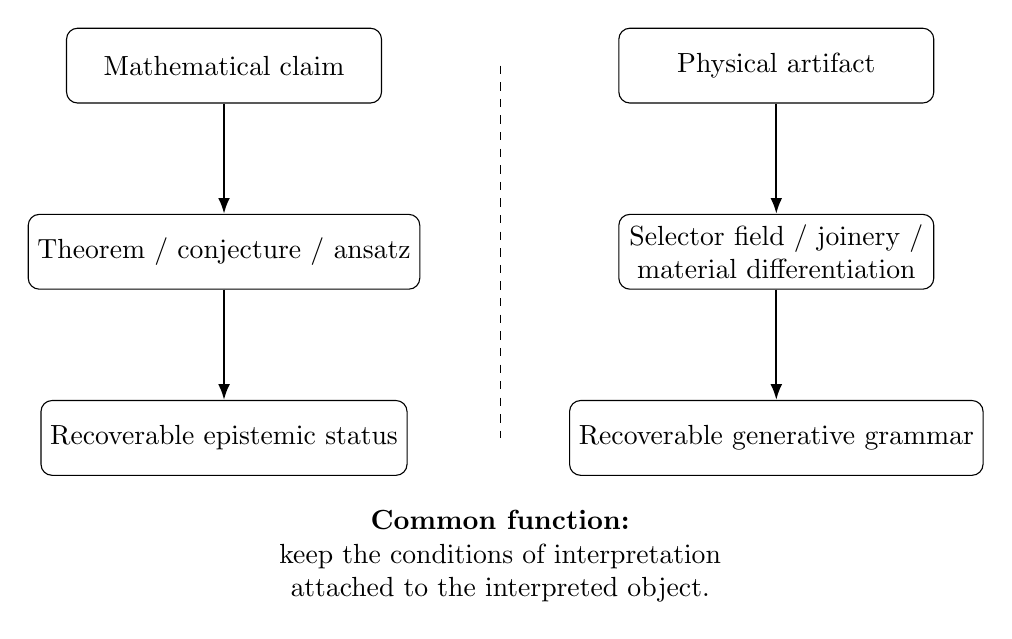
\begin{tikzpicture}[
    node distance=1.4cm and 2.5cm,
    box/.style={draw, rounded corners, align=center,
                minimum width=4.0cm, minimum height=0.95cm},
    arr/.style={-{Latex[length=2mm]}, thick}
]

\node[box] (claim) {Mathematical claim};
\node[box, below=of claim] (status)
    {Theorem / conjecture / ansatz};
\node[box, below=of status] (reader)
    {Recoverable epistemic status};

\draw[arr] (claim) -- (status);
\draw[arr] (status) -- (reader);

\node[box, right=3.0cm of claim] (artifact)
    {Physical artifact};
\node[box, below=of artifact] (selector)
    {Selector field / joinery /\\material differentiation};
\node[box, below=of selector] (grammar)
    {Recoverable generative grammar};

\draw[arr] (artifact) -- (selector);
\draw[arr] (selector) -- (grammar);

\draw[dashed] ($(claim)!0.5!(artifact)$)
    -- ($(reader)!0.5!(grammar)$);

\node[below=0.8cm of $(reader)!0.5!(grammar)$, align=center]
    {\textbf{Common function:}\\
     keep the conditions of interpretation\\
     attached to the interpreted object.};

\end{tikzpicture}
\caption{Epistemic marking and hyperpleonastic legibility as parallel forms of structural honesty. A theorem label preserves claim status; a selector field preserves access to generative status.}
\label{fig:labels-selectors}
\end{figure}

\section{Recoverable Information Density: A Quantitative Analogue}

Hyperpleonastic legibility also supplies something the earlier, more purely epistemic sections could only gesture toward: a quantitative treatment of degree rather than a binary judgment of honest or dishonest. Given bounded observation $O$ of an artifact and its generative grammar $G$, the recoverable information is the mutual information $I_{\mathrm{recoverable}} = I(O;G)$, and the recoverable information density is the ratio

\[
\mathrm{RID} = \frac{I_{\mathrm{recoverable}}}{I_{\mathrm{total}}}.
\]

An artifact can therefore be physically present, fully functional, and yet carry almost none of the information needed to recover the grammar responsible for its own construction; conversely, a high-RID artifact preserves substantial interpretive structure within its own material substrate, independent of any external authority. This measure should not be mistaken for a general-purpose metric of structural honesty across every domain considered in this essay; it is a specific quantity defined for recoverable generative information in physical artifacts. Its value here is illustrative: it demonstrates that the abstract principle of recoverable warrant admits at least one rigorous, gradated formalization rather than remaining only a qualitative injunction.

\section{Layered Interpretability: Expertise Should Refine Rather Than Reverse}

A further concept from the same material theory extends structural honesty across scales of observation. Consider nested observational resolutions $O_1 \subset O_2 \subset O_3$, corresponding, for instance, to what a novice, a measuring instrument, and a specialist can each recover about an artifact. The theory of hyperpleonastic legibility requires monotonic refinement across these resolutions: additional observational capacity should increase the specificity of an interpretation without contradicting whatever interpretation was already available at a coarser resolution. A novice's coarse classification, a technician's parameter measurement, and a specialist's recovery of lineage or calibration history should stand in a relation of successive refinement, not successive correction.

Generalized beyond physical artifacts, this becomes a principle of epistemic monotonicity: a structurally honest representation should, wherever possible, allow increasing expertise to refine a warranted interpretation rather than reveal that the simpler presentation was fundamentally misleading. This has direct application to abstracts, diagrams, model cards, documentation, mathematical notation, and user interfaces, all of which can be evaluated by whether their simplified presentation constitutes a valid coarse-graining of the underlying structure or merely a convenient falsehood that experts are left to unlearn later.

\begin{figure}[ht]
\centering
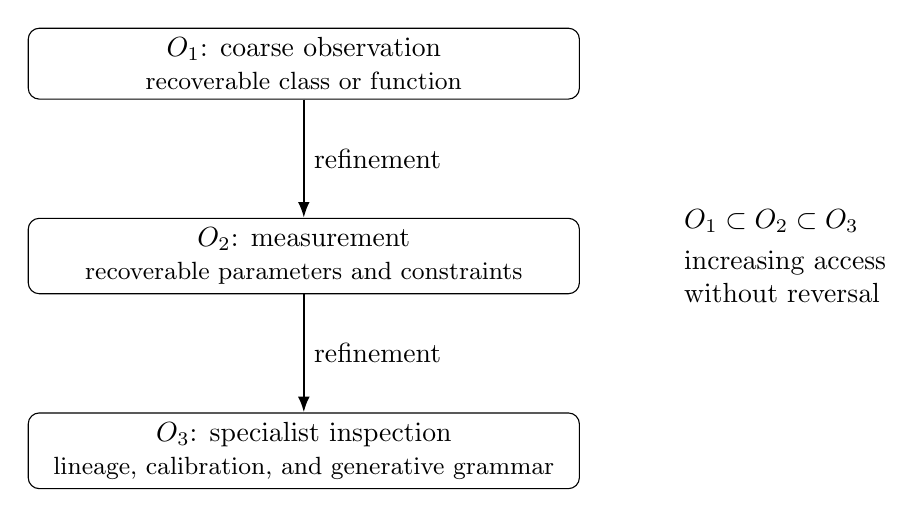
\begin{tikzpicture}[
    node distance=1.5cm,
    box/.style={draw, rounded corners, align=center,
                minimum width=7.0cm, minimum height=0.9cm},
    arr/.style={-{Latex[length=2mm]}, thick}
]

\node[box] (o1)
    {$O_1$: coarse observation\\
     \small recoverable class or function};

\node[box, below=of o1] (o2)
    {$O_2$: measurement\\
     \small recoverable parameters and constraints};

\node[box, below=of o2] (o3)
    {$O_3$: specialist inspection\\
     \small lineage, calibration, and generative grammar};

\draw[arr] (o1) -- node[right] {refinement} (o2);
\draw[arr] (o2) -- node[right] {refinement} (o3);

\node[right=1.2cm of o2, align=left]
    {$O_1 \subset O_2 \subset O_3$\\[3pt]
     increasing access\\
     without reversal};

\end{tikzpicture}
\caption{Monotonic interpretability. Increased observational capacity should refine a warranted coarse interpretation rather than reveal that the earlier representation was fundamentally misleading.}
\label{fig:monotonic-interpretability}
\end{figure}

The caption above is deliberately precise, because this is not a claim that every expert conclusion must agree with every novice conclusion. The condition concerns a representation deliberately designed to expose itself at multiple resolutions: its coarse reading should be a legitimate coarse-graining rather than misinformation.

This can be stated more precisely in the vocabulary already introduced for TARTAN below. Let $\mathcal{F}$ assign to each observational resolution the interpretations recoverable at that resolution, and let $\rho_{21}: \mathcal{F}(O_2) \to \mathcal{F}(O_1)$ be the map that forgets the detail distinguishing $O_2$ from $O_1$. Monotonic interpretability requires that the coarse presentation $s_1 \in \mathcal{F}(O_1)$ actually lie in the image of the true underlying state under $\rho_{21}$, rather than being an independently constructed surrogate $s_1' \notin \mathrm{Im}(\rho_{21})$ that merely happens to resemble a legitimate coarse-graining. A surrogate of this kind is not a simplification of the finer interpretation; it is a different claim wearing the finer interpretation's coarse appearance.

\section{Compositional Dishonesty: When Every Part Is True}
\label{sec:composition}

Structural dishonesty can arise without any dishonest component. This is stronger than the observation that a representation may contain individually correct labels arranged into a misleading diagram. The same failure occurs in arguments, datasets, summaries, interfaces, and institutional reporting whenever individually warranted elements are composed in a manner that silently introduces an unwarranted relation among them.

Suppose a representation contains claims $c_1,\ldots,c_n$, each independently warranted:

\[
W(c_i) \qquad \text{for every } i.
\]

It does not follow that an arbitrary composition

\[
C(c_1,\ldots,c_n)
\]

inherits warrant merely because all of its components do. Composition itself is an operation with epistemic content. Ordering can imply causation; juxtaposition can imply comparison; common scale can imply commensurability; aggregation can imply that omitted variation is irrelevant; a shared heading can imply membership in a common reference class. None of these relations is guaranteed by the truth of the components.

Thus

\[
\boxed{
\bigwedge_i W(c_i)
\not\Rightarrow
W\!\left(C(c_1,\ldots,c_n)\right).
}
\]

The composition requires its own bridge principle.

This explains how a document can contain no false sentence and nevertheless produce a false understanding. Selective chronology may imply a causal sequence without stating one. A benchmark table may place incomparable measurements in adjacent columns and thereby imply a ranking no measurement actually warrants. A dashboard may aggregate heterogeneous failures into a single success percentage whose apparent precision exceeds the meaning of its inputs. A generated image may contain individually plausible hands, tools, shadows, vegetation, and architecture while their joint configuration has no coherent generating world.

Compositional dishonesty is therefore not reducible to omission. The omitted object is often a relation rather than a fact: the warrant for putting these particular elements together in this particular way. This observation provides a direct transition to the local-to-global problem. TARTAN can be read as a formal account of one especially important compositional failure: locally admissible sections do not automatically warrant the global object their juxtaposition appears to promise.

\section{TARTAN and Constraint Closure: Local Honesty Does Not Guarantee Global Honesty}

The TARTAN framework supplies a mathematical model of the same phenomenon in a different register. A collection of locally acceptable statements need not glue into a single globally realizable whole; a persistent nonzero $H^1$ obstruction, or a failure of descent, marks precisely the cases where local coherence cannot be honestly reported as global realization. Hyperpleonastic legibility itself eventually adopts the same sheaf-theoretic vocabulary for a different purpose, treating locally recoverable interpretations of instruction fragments, drawn from bounded observation patches of an artifact, as sections that must agree on overlaps and glue to a global interpretation of the object's grammar. The two applications converge on the same prohibition:

\[
\boxed{\text{local legibility} \not\Rightarrow \text{global coherence.}}
\]

Constraint Closure generalizes the point beyond any sheaf-theoretic apparatus. A system can satisfy every constraint expressed within its own representation while that representation remains inadequate to the world it is meant to describe. The distinction between representational closure and semantic or physical closure matters precisely because a closed model cannot use its own internal consistency as evidence that nothing relevant lies outside the closure. Passing every test a system sets for itself is not the same achievement as being adequate to what the tests were meant to assess.

\section{Diagnostic Coordinates: Legibility Does Not Yet License Intervention}
\label{sec:diagnostic}

The Diagnostic Coordinates framework governs the transition from representation to action, and it becomes considerably sharper once the material discussion above is in view. Recovering an artifact's generative grammar, or diagnosing a discrepancy in a formal system, increases the information available for intervention, but availability of that information does not by itself establish that any particular intervention is warranted. The relevant sequence is:

\[
\text{legibility} \not\Rightarrow \text{detection} \not\Rightarrow \text{diagnosis} \not\Rightarrow \text{reference-class selection} \not\Rightarrow \text{repair warrant}.
\]

Each arrow in this sequence requires its own independent justification. A detected deviation from expectation is evidence about a discrepancy; it is not, on its own, a license to correct it. The admissible reference class against which a system's behavior is being judged must itself be independently grounded, the structural consequences of a proposed intervention must be considered, uncertainty and irreversible risk must be represented honestly, and the null intervention, doing nothing, must remain visibly available as a live option rather than being displaced by the mere existence of a diagnosis. This is an important constraint on any overly simple notion of a right to repair: the capacity to see what could be changed about a system is a separate achievement from possessing warrant to change it, and structural honesty requires that the two never be silently conflated.

\section{Provenance: The Endpoint Cannot Testify for Its History}
\label{sec:provenance}

A further generalization concerns time. The Chain of Memory framework, the treatment of irreversible events in Spherepop, trajectory-first ontology, and the analysis of originality and reproduction all reject a single, tempting inference: that two states sharing a present configuration must share a relevant history. Formally, $x(t) = y(t)$ does not imply $x \sim y$ with respect to provenance, responsibility, identity, admissibility, or legitimate continuation. Hyperpleonastic legibility provides a striking material instance of the same idea: traditional artifacts often carry legible traces of their own generative history directly in their form, as when joinery exposes assembly sequence, fiber orientation indicates load-bearing direction, or fastener geometry reveals the intended order of disassembly. Such an object does not merely function; it also, to a recoverable degree, testifies to how it came to be as it is.

The corresponding failure is historical overclaiming: allowing a present state to imply, by its silence, a history that its representation has in fact discarded. A corrected result that is presently accurate but silently omits an earlier failed attempt is dishonest in exactly this sense, even though every currently visible claim is true. Structural honesty therefore requires that relevant histories remain recoverable wherever they bear on the interpretation, admissibility, or trustworthiness of a present state; an endpoint must not be permitted to impersonate the trajectory that produced it.

\section{Synthetic Provenance: When the Artifact Manufactures Its Own History}
\label{sec:synthetic}

Everything discussed so far concerns a real history that is subsequently lost, compressed, or silently omitted. A more radical failure is available once an artifact's apparent history need not have occurred at all. Ordinary compression follows

\[
H \longrightarrow C(H),
\]

a rich generating history compressed into an artifact from which that history becomes progressively harder to recover. Synthetic imagery of the kind now common on social media inverts this relation, though not quite in the way it first appears. An image-generation system does not produce an artifact with no generating history; it produces an artifact $A$ with a genuine computational generating history $H_G$, the prompt, model, seed, sampler, and inference environment that actually produced these pixels, but without the depicted historical process $H_D$ that an observer would ordinarily infer from the image: a child's afternoon spent constructing a sculpture, a diagnosis and its treatment. A publisher may then attach a fabricated depicted history $\widehat H_D$ after the fact:

\[
H_G \longrightarrow A \longrightarrow \widehat H_D, \qquad H_D = \varnothing.
\]

The artifact therefore has provenance. It simply does not have the provenance it appears to testify to.

This licenses a distinction the essay has not needed until now. An artifact's generative provenance $H_G(A)$, the causal process that actually produced it, need not coincide with its depicted provenance $H_D(A)$, the history the artifact invites an observer to infer:

\[
H_G(A) \neq H_D(A).
\]

For an ordinary documentary photograph, ideally $H_D \subseteq H_G$, since the photographed event genuinely participates in the causal chain that produced the photograph. For the synthetic images considered here, $H_D \cap H_G \approx \varnothing$: the depicted child did not build the depicted sculpture, and neither child nor sculpture need have existed, while the artifact's actual generating history, a model's inference pass, is concealed rather than depicted. This is stronger than missing provenance. It is provenance substitution. A caption describing hours spent building a matchstick sculpture, or a letterboard reporting a child's recovery from illness, does not compress anything; it fabricates the one component of provenance, $H_D$, that the generation process left empty.

For the ordinary compression case discussed throughout this essay,

\[
\boxed{\text{provenance loss} \;\Rightarrow\; \text{repair entropy} \;\Rightarrow\; \text{narrative substitutability}}
\]

remains correct: a real $H$ existed and was discarded. Synthetic media introduces a distinct operation on top of it:

\[
\boxed{\text{concealed generative provenance} + \text{fabricated depicted provenance} \;\Rightarrow\; \text{provenance substitution}.}
\]

This sharpens the connection to Attestal noted in Section~\ref{sec:attestal}: \texttt{Attested<T>} preserves $H_G$ specifically so that an artifact cannot silently acquire an incompatible $H_D$. Retaining ``simulation'' alongside a numerical result exists precisely to prevent someone from later substituting ``photonic hardware experiment'' as the result's depicted history.

Once $H_D$ has been destroyed or fabricated, the absence functions as a degree of freedom into which any sufficiently plausible history can be inserted, and many mutually incompatible histories become simultaneously compatible with the surviving artifact. The audience is shown a plausible endpoint and infers, in the ordinary direction $A \Rightarrow H_D$, that the depicted history must have happened. No history was compressed. The depicted history simply never existed.

A further diagnostic becomes available once this pattern is recognized at scale, and it is considerably harder to fake than any single image. A genuine historical event is singular: one child, one recovery, one photograph. A generative template is not singular in this way, and its outputs betray the fact by appearing as a population of variants rather than a single artifact. When the same narrative, a child holding a letterboard announcing recovery from illness, or a craftsman posing beside a wooden model, recurs across a population of posts while demographic appearance, clothing, setting, and other particulars vary systematically, the population itself supplies evidence unavailable from any single image: no single historical event can have hundreds of mutually exclusive concrete instantiations, so the variation is not evidence of many similar real events but evidence that a generative template has been sampled repeatedly. This gives a usable test distinct from anything internal to a single image: where the claimed history entails a unique event, the appearance of the same narrative attached to a population of incompatible particulars is evidence against the narrative's central presupposition, regardless of how convincing any individual instance looks in isolation. Call this the variant-multiplicity test. It has the same logical shape as the local-to-global failures discussed in connection with TARTAN: no single instance need be locally implausible for the population as a whole to be globally inadmissible.

A second, weaker diagnostic remains available even for a single image viewed in isolation, precisely because provenance has been substituted rather than merely hidden. Once historical warrant is absent, physical consistency becomes the last remaining check: whether a shadow is cast by a light source consistent with the rest of the scene, whether an object shares a focal plane and scale with the figure beside it, whether foliage native to one climate appears beside architecture native to another. These are not reliable in general, since a sufficiently careful synthesis or a sufficiently ordinary coincidence can satisfy them, but their violation is informative in the same direction as the variant-multiplicity test: both are attempts to recover, from the artifact alone, constraints that a genuine depicted history would have imposed automatically and that a fabricated one imposes only accidentally.

The harm involved is not only epistemic. A generated image of a child's craft project competes for exactly the same attention as a photograph of a real child's craft project, and the generated version can be produced, captioned, and reposted at a volume and emotional calibration no single real event can match. This is a distributional failure rather than a representational one: it is not that the synthetic post misrepresents anything about a particular real child, but that its existence, repeated at scale, absorbs the collective attention that would otherwise have been available to real instances of the same hardship or craft. A real child's carefully made bottle-cap sculpture is not defeated by a false claim about it; it is defeated by never being seen at all, because the attention economy has been saturated by an unlimited supply of emotionally optimized synthetic competitors. This connects directly to the distinction introduced earlier under dimensional poverty, existence not implying availability, and availability not implying recoverability, but names a distinct failure: here the artifact is fully recoverable and the history is entirely absent, yet the harm falls on an unrelated, structurally similar artifact that possessed a genuine history all along and was simply outcompeted for visibility.

None of this requires a new branch of the theory. Provenance substitution is the limiting case of the promotion half of Figure~\ref{fig:promotion-externalization}: externalization destroys warrant that existed, while promotion manufactures warrant that did not. Here the manufactured warrant takes the specific form of a depicted history, and the asserted $\widehat H_D$ has essentially no support in the artifact's actual causal history $H_G$. Synthetic provenance is not an anomalous case requiring separate treatment; it is what promotion looks like when the weaker relation being promoted from is empty.

\section{Unknown Provenance Is Not Fabricated Provenance}
\label{sec:unknown-provenance}

The synthetic-provenance argument requires one further distinction. Failure to possess a provenance record is not itself evidence that provenance has been fabricated. An old photograph discovered without a caption, an undocumented tool found in a workshop, or a numerical result separated from its laboratory notebook may have perfectly genuine histories that are no longer recoverable. Structural honesty requires that this uncertainty remain uncertainty.

Let $H$ denote the actual history of an artifact and let $\mathcal{H}(A)$ be the set of histories still compatible with the evidence available from $A$ and its legitimate context. When provenance has merely been lost,

\[
H \in \mathcal{H}(A),
\qquad
|\mathcal{H}(A)| > 1,
\]

but the observer does not know which member is actual. The honest claim is therefore set-valued: the evidence constrains history to some admissible family without selecting a unique member.

Fabricated provenance performs a different operation. It selects some

\[
\widehat H \in \mathcal{H}(A)
\]

and presents

\[
\widehat H = H
\]

without possessing the warrant required to collapse the admissible set to that single history. Synthetic provenance may be stronger still when the asserted history is incompatible with the artifact's authenticated generating record.

This yields an important principle:

\[
\boxed{
\text{underdetermination must remain visible as underdetermination.}
}
\]

Structural honesty therefore does not demand omniscience. Quite the opposite: it supplies a principled representation for ignorance. ``Unknown,'' ``one of these histories,'' ``not independently verified,'' and ``provenance lost'' are not defects to be cosmetically repaired. They are positive epistemic states whose preservation prevents narrative substitutability from becoming narrative assertion.

The distinction is especially important for archival practice. A provenance system that refuses to represent missing information will tend to manufacture defaults, inferred metadata, or plausible reconstructions simply to maintain a complete schema. A structurally honest archive must instead permit holes in its own structure. An explicit unknown is more informative than an invented certainty because it preserves the location at which future evidence could still perform genuine repair.

\section{Compression, Compressive Capture, and the Right to Forget}

Every useful abstraction discards information, and structural honesty cannot sensibly demand perfect preservation; the relevant question is always whether the discarded distinctions remain irrelevant to whatever operations are subsequently performed on the compressed representation. For an abstraction $A: X \to Y$ with $A(x_1) = A(x_2)$, the treatment of $x_1$ and $x_2$ as equivalent is legitimate only relative to a context in which the difference between them does not matter. Should that difference later become causally, diagnostically, or normatively significant, continuing to treat $x_1$ and $x_2$ as interchangeable exceeds the warrant the abstraction actually possesses. This yields one of the more compact formulations available in this territory:

\begin{quote}
An abstraction must earn the right to forget.
\end{quote}

Hyperpleonastic legibility supplies a material and political-economic counterpart to this principle under the heading of compressive capture. As a manufacturing or design process is optimized, the tolerance manifold available to it typically contracts, $\dim(T) \downarrow$, while the generative grammar responsible for the resulting artifacts is increasingly externalized into proprietary or otherwise inaccessible authorities. The artifact that results can become simultaneously more efficient, more uniform, and less interpretable, with recoverable information tending toward zero even as the total generative information required to produce it remains high. This distinction allows a sharper separation than the word compression alone provides. Legitimate compression discards distinctions that have been shown to be irrelevant to the operations the representation must support. Dishonest compression discards distinctions while continuing to depend on them elsewhere, or relocates them into an authority inaccessible to whoever is left holding the compressed interface, while nonetheless presenting that interface as sufficient.

\section{Dimensional Poverty: Structural Honesty as Distributed Interpretive Authority}

A brief but important extension concerns who, rather than merely whether, can recover a given structure. Opacity does not simply remove information from circulation; it redistributes interpretive power. Hyperpleonastic legibility defines dimensional poverty as the contraction of the control surface available to an artifact's users for local repair, substitution, and autonomous operation, and observes that a society can possess technologically sophisticated artifacts while the great majority of its members possess very little access to the generative structure underlying them. Structural honesty therefore has an irreducibly distributional dimension: it is not sufficient that the relevant structure exist somewhere in the world. A server holding perfect documentation does not render an artifact structurally transparent to an agent who has been denied access to that server. This connects directly to an earlier distinction concerning preservation and reachability, and yields a three-part refinement of the general principle:

\[
\boxed{\text{existence} \not\Rightarrow \text{availability} \not\Rightarrow \text{recoverability.}}
\]

\section{Admissibility: Recoverability Is Not Permission}

The Admissibility Program supplies a necessary counterweight, preventing the argument from collapsing into an undiscriminating demand for maximal transparency everywhere. Not every distinction needs to be preserved in every context; not every piece of information needs to be exposed to every observer; not every physically or computationally available operation is thereby admissible. The distinction that matters is narrower and more precise: whether the information required to evaluate a given operation remains available to the agents actually responsible for evaluating it. The general prohibition inherited from the admissibility work,

\[
\text{possibility} \not\Rightarrow \text{permission},
\]

applies here just as it applies to intervention in the diagnostic framework above. The task structural honesty sets is therefore not indiscriminate disclosure but warrant-preserving selective compression: discarding what may safely be discarded, and keeping recoverable what continues to bear on legitimate evaluation.

\section{Auditability: Recoverability Must Survive Challenge}
\label{sec:auditability}

Recoverable warrant is stronger than stored warrant. A system may retain every piece of information needed to justify a claim and nevertheless arrange that information so that no realistic observer can retrieve, associate, or evaluate it when the claim is challenged. Structural honesty therefore requires an operational notion of recoverability rather than mere archival existence.

Let $J(c)$ denote the justificatory structure supporting claim $c$. To say that $J(c)$ exists is only to assert preservation. To say that it is recoverable requires, relative to some legitimate evaluator $a$ and bounded resources $B$, that there exist an admissible retrieval procedure

\[
\mathcal{R}(a,c,B) \longrightarrow J(c)
\]

with sufficient fidelity for the evaluator to determine whether $J(c)$ really licenses $c$. A provenance record encrypted under an unavailable key, a citation pointing to a vanished dataset, a billion-entry audit log with no index connecting events to claims, or documentation legally inaccessible to the person expected to repair an artifact may all preserve information while failing this stronger condition.

This distinction gives structural honesty a temporal dimension. Warrant must not merely accompany a claim at the moment of production; the association must survive the transformations through which the claim later passes. Copying, summarization, format conversion, model training, database migration, aggregation, publication, and archival storage can each preserve the visible claim while severing the path back to its justification.

One may therefore distinguish three increasingly strong conditions:

\[
\text{preserved warrant}
\;\not\Rightarrow\;
\text{reachable warrant}
\;\not\Rightarrow\;
\text{auditable warrant.}
\]

Preservation means that the relevant structure still exists. Reachability means that the legitimate evaluator can obtain it. Auditability means that the connection between warrant and claim remains sufficiently structured to test the promotion the claim embodies.

This is where structural honesty becomes more than a virtue of initial representation. It becomes a property of an information lifecycle. A claim whose warrant predictably disappears on export, compression, quotation, or aggregation is only temporarily honest. The stronger requirement is that honesty survive transport.

\section{Refusal: The Preservation of Unresolved Structure}

The Autonomy of Refusal supplies the operational terminus toward which every preceding section has been building. Each of the frameworks discussed above specifies circumstances under which one relation must not be silently promoted into a stronger one; refusal is what a system does when it is asked, or pressured, to perform exactly that promotion anyway. When the evidence available does not warrant promoting a conjecture to a theorem, the conjecture remains a conjecture. When diagnostic information does not establish repair warrant, the null intervention remains available and legitimate. When a compressed representation has discarded information required for responsible continuation, uncertainty may not be replaced by a fabricated decision merely because the surrounding procedure demands some output. And, in the material register introduced by hyperpleonastic legibility, an artifact's refusal to become mute, its preservation of enough structured variation that its interpretation does not collapse entirely into dependence on an external institutional key, is itself a species of the same act.

This yields a three-part statement of refusal that draws the epistemic, operational, and material strands of the essay together:

\begin{quote}
Epistemic refusal: do not claim what has not been established.\\
Operational refusal: do not perform what has not been warranted.\\
Material refusal: do not erase the structure required for future interpretation.
\end{quote}

These are not three different principles but three settings in which a single boundary-preserving operation is required. Refusal is not opposition to action in general; it is epistemic honesty exercised under pressure to act.

\section{Structural Dishonesty Without Lying}

It is worth pausing to state explicitly a distinction implicit throughout the preceding sections, because the word honesty invites a psychological reading that this essay does not intend. Structural dishonesty does not require deception, and it does not require that any individual statement be false. A benchmark can report every number with perfect accuracy and still overstate what has actually been measured. A diagram can use only legitimate technical labels while its spatial arrangement implies relationships the underlying structure does not support. A model card can consist entirely of true statements while nonetheless obscuring the limitations that matter most for a given use. An artifact can function correctly in every respect that a casual inspection would test while having had its generative grammar entirely externalized to an authority its user cannot reach. In each case, no one need have lied.

This motivates a tripartite distinction that considerably reduces the risk of the term being misread. Truth is a property of propositions considered against the world. Sincerity is a property of agents considered against their own beliefs. Structural honesty is a property of the relationship between a representation's apparent warrant and the warrant its supporting structure actually provides. A person or a system can be entirely sincere, and every individual claim it makes can be entirely true, while the structure of its representations remains dishonest in this third, distinct sense.

\section{Why Structural Honesty Is Not Transparency}
\label{sec:not-transparency}

Structural honesty should not be identified with transparency. Transparency concerns visibility: whether information has been disclosed or made available. Structural honesty concerns calibration: whether the apparent strength of a representation remains proportionate to the warrant available for it. The two can therefore come apart.

A system may be highly transparent and structurally dishonest. It may publish its source code, datasets, logs, assumptions, and intermediate calculations while still drawing a conclusion those materials do not license. Nothing is hidden; the promotion is simply invalid. Conversely, a system may legitimately withhold information for reasons of privacy, security, confidentiality, or irrelevance while remaining structurally honest, provided that the resulting claims do not imply warrant that depends upon the inaccessible material in a way the relevant evaluator is expected simply to trust.

The distinction is therefore:

\[
\text{transparency}: \quad \text{Can the structure be seen?}
\]
\[
\text{structural honesty}: \quad
\text{Does the representation claim only what its structure warrants?}
\]

Transparency can support structural honesty by making warrant auditable, but it is neither necessary in every context nor sufficient in any context. A thousand pages of disclosed evidence do not license a conclusion that does not follow from them. Structural honesty concerns the validity of the bridge, not merely whether the bridge is visible.

\section{The Architecture of Structural Honesty}

The essay's argument has moved through a specific progression: status, promotion, bridge, warrant budget, composition, provenance, underdetermination, compression, auditability, admissibility, refusal. Each stage answers a question the previous stage leaves open. Status marking asks what kind of claim is being made; the bridge principle asks what would license moving to a stronger kind; the warrant budget asks where an apparent increase in strength actually came from; composition asks whether truth at the level of parts survives assembly into a whole; provenance and its underdetermined and synthetic variants ask what history a representation may honestly claim; auditability asks whether that history remains reachable under challenge rather than merely stored; and admissibility and refusal ask what follows once warrant has genuinely run out.

The frameworks surveyed above are not renamed instances of a single underlying theory; each retains its own distinct content, developed for its own reasons. What they share is a recurring methodological invariant, visible once the frameworks are placed side by side:

\[
\begin{array}{lll}
\text{Epistemic status marking} & : & \text{conjecture} \not\Rightarrow \text{theorem} \\
\text{Bridge Principles} & : & R_0 \text{ (no adequate } B\text{)} \not\Rightarrow R_1 \\
\text{Attestal} & : & \text{simulation} \not\Rightarrow \text{hardware execution} \\
\text{Representational Constraint / MAGI} & : & \text{plausibility} \not\Rightarrow \text{truth} \\
\text{Hyperpleonastic Legibility} & : & \text{function} \not\Rightarrow \text{legibility} \\
\text{Compositional Dishonesty} & : & \textstyle\bigwedge_i W(c_i) \not\Rightarrow W(C(c_1,\ldots,c_n)) \\
\text{TARTAN / Constraint Closure} & : & \text{local coherence} \not\Rightarrow \text{global coherence} \\
\text{Diagnostic Coordinates} & : & \text{detection} \not\Rightarrow \text{repair warrant} \\
\text{Chain of Memory / Spherepop} & : & \text{endpoint} \not\Rightarrow \text{history} \\
\text{Synthetic Provenance} & : & \text{plausible history} \not\Rightarrow \text{actual history} \\
\text{Compression--Repair} & : & \text{reconstruction} \not\Rightarrow \text{preservation} \\
\text{Auditability} & : & \text{preserved warrant} \not\Rightarrow \text{auditable warrant} \\
\text{Dimensional Poverty} & : & \text{existence} \not\Rightarrow \text{recoverability} \\
\text{Admissibility Program} & : & \text{possibility} \not\Rightarrow \text{permission} \\
\text{Autonomy of Refusal} & : & \text{demand for continuation} \not\Rightarrow \text{obligation to continue.}
\end{array}
\]

Seen this way, structural honesty is not another framework standing beside RSVP, TARTAN, the admissibility program, Spherepop, Chain of Memory, MAGI, Diagnostic Coordinates, hyperpleonastic legibility, and refusal. It is the methodological invariant that explains why the same kind of boundary keeps reappearing, independently motivated, across all of them.

\begin{figure}[H]
\centering
\resizebox{0.92\textwidth}{!}{%
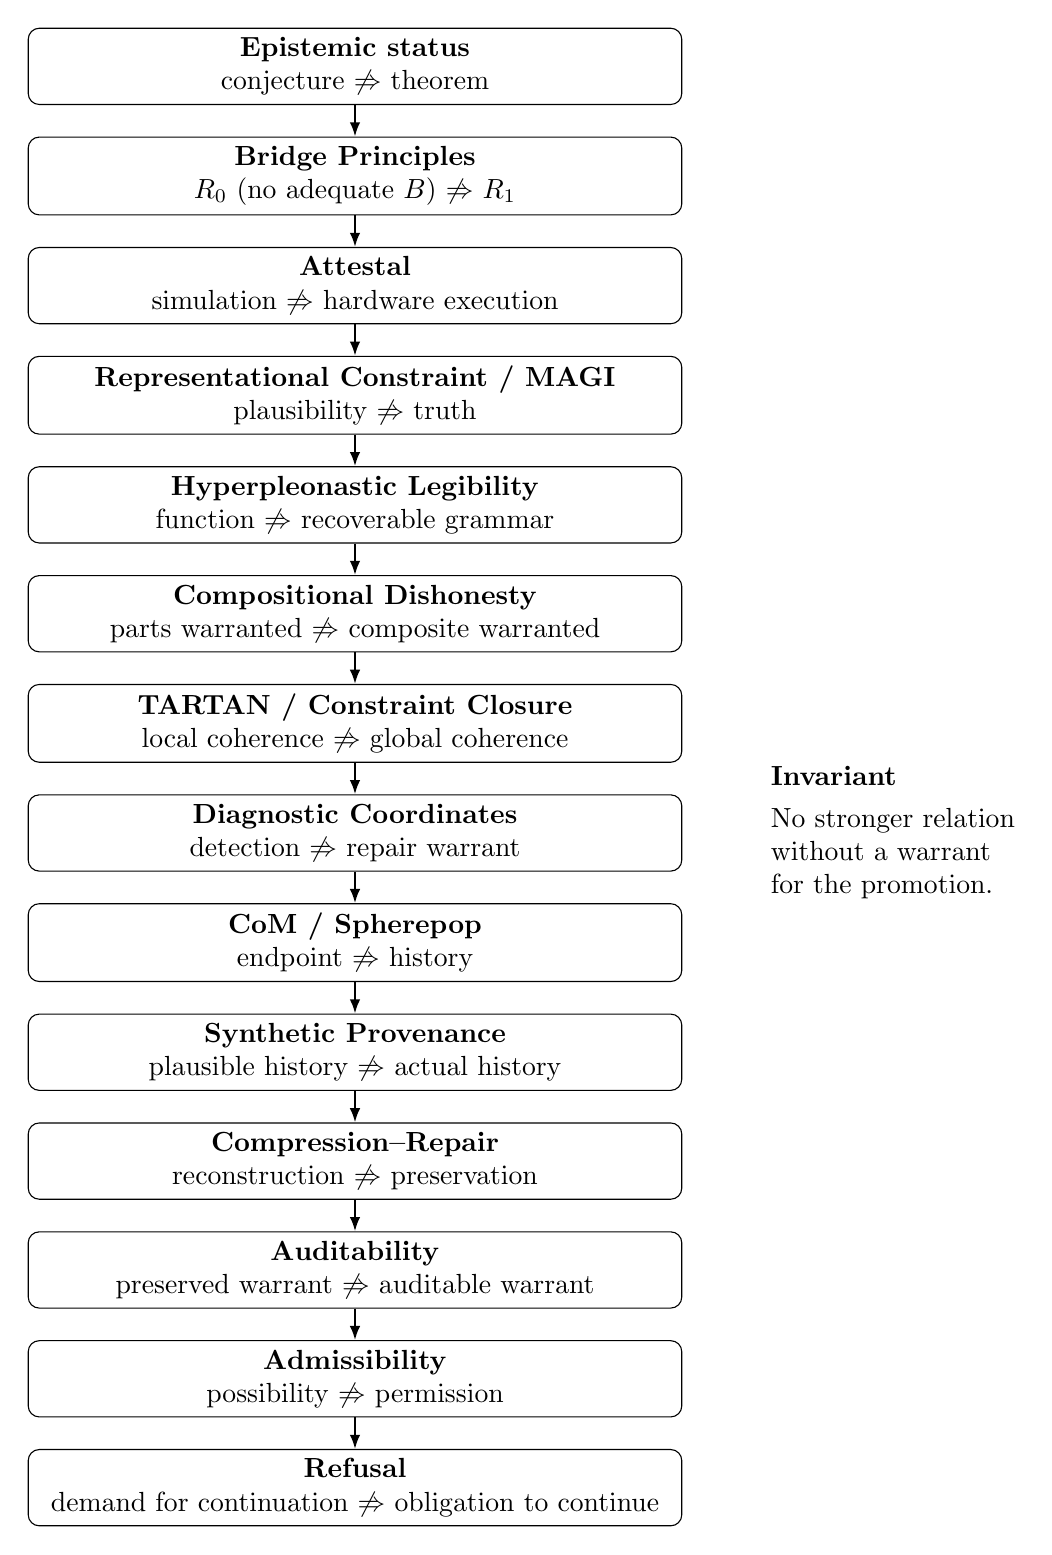
\begin{tikzpicture}[
    node distance=0.4cm,
    box/.style={draw, rounded corners, align=center,
                minimum width=8.3cm, minimum height=0.6cm},
    arr/.style={-{Latex[length=1.8mm]}, thick}
]

\node[box] (ep)
    {\textbf{Epistemic status}\\
     conjecture $\not\Rightarrow$ theorem};

\node[box, below=of ep] (bridge)
    {\textbf{Bridge Principles}\\
     $R_0$ (no adequate $B$) $\not\Rightarrow$ $R_1$};

\node[box, below=of bridge] (att)
    {\textbf{Attestal}\\
     simulation $\not\Rightarrow$ hardware execution};

\node[box, below=of att] (rep)
    {\textbf{Representational Constraint / MAGI}\\
     plausibility $\not\Rightarrow$ truth};

\node[box, below=of rep] (hyp)
    {\textbf{Hyperpleonastic Legibility}\\
     function $\not\Rightarrow$ recoverable grammar};

\node[box, below=of hyp] (compo)
    {\textbf{Compositional Dishonesty}\\
     parts warranted $\not\Rightarrow$ composite warranted};

\node[box, below=of compo] (tar)
    {\textbf{TARTAN / Constraint Closure}\\
     local coherence $\not\Rightarrow$ global coherence};

\node[box, below=of tar] (diag)
    {\textbf{Diagnostic Coordinates}\\
     detection $\not\Rightarrow$ repair warrant};

\node[box, below=of diag] (hist)
    {\textbf{CoM / Spherepop}\\
     endpoint $\not\Rightarrow$ history};

\node[box, below=of hist] (syn)
    {\textbf{Synthetic Provenance}\\
     plausible history $\not\Rightarrow$ actual history};

\node[box, below=of syn] (comp)
    {\textbf{Compression--Repair}\\
     reconstruction $\not\Rightarrow$ preservation};

\node[box, below=of comp] (audit)
    {\textbf{Auditability}\\
     preserved warrant $\not\Rightarrow$ auditable warrant};

\node[box, below=of audit] (adm)
    {\textbf{Admissibility}\\
     possibility $\not\Rightarrow$ permission};

\node[box, below=of adm] (refu)
    {\textbf{Refusal}\\
     demand for continuation $\not\Rightarrow$ obligation to continue};

\foreach \a/\b in {ep/bridge,bridge/att,att/rep,rep/hyp,hyp/compo,compo/tar,tar/diag,diag/hist,hist/syn,syn/comp,comp/audit,audit/adm,adm/refu}{
    \draw[arr] (\a) -- (\b);
}

\node[right=1.0cm of diag, align=left]
    {\textbf{Invariant}\\[3pt]
     No stronger relation\\
     without a warrant\\
     for the promotion.};

\end{tikzpicture}%
}
\caption{Structural honesty as a methodological invariant across the research program. The frameworks differ in subject matter, but each preserves a boundary between a weaker relation and an unwarranted stronger one.}
\label{fig:architecture}
\end{figure}

The vertical progression in Figure~\ref{fig:architecture} carries an intellectual meaning of its own. It begins with the almost trivial scholarly discipline of not calling a conjecture a theorem, then moves through representation and physical legibility, through global coherence and intervention, into history and compression, and finally arrives at admissibility and refusal. It reproduces visually what the preceding sections have argued in prose: structural honesty was not introduced wholesale as a new framework: the same constraint kept reappearing at progressively deeper levels of the research program.

\section{Conclusion: A Claim Must Earn Its Strength}

The argument of this essay began with a habit too small to seem worth naming: writing the word conjecture rather than the word theorem. What that habit turns out to express, once traced outward through representation, locality, intervention, provenance, compression, and material artifacts, is a single, demanding commitment. A theorem must earn its status. A model must earn its interpretation. A global claim must earn its passage from local evidence. A repair must earn the intervention it performs. An abstraction must earn the distinctions it discards. An artifact must earn the confidence its smooth functioning invites. A continuation must earn its own admissibility.

The essay's two central formulations can now be stated together, as they were always meant to be read:

\[
\boxed{\text{A claim must earn the strength of its assertion.}}
\]
\[
\boxed{\text{An abstraction must earn the right to forget.}}
\]

And a third, added by the material argument of the middle sections, belongs beside them:

\[
\boxed{\text{An artifact must earn the confidence its function invites.}}
\]

A fourth, added by the discussion of synthetic provenance, closes the set:

\[
\boxed{\text{An artifact must not testify to a history it did not have.}}
\]

A fifth, supplied by the bridge principle and the warrant budget, is arguably the deepest of the five, since it is the only one phrased as a positive requirement rather than a prohibition, and it is what makes the theory compatible with genuine discovery rather than merely hostile to overstatement:

\[
\boxed{\text{Every increase in epistemic strength must have a traceable source.}}
\]

A conjecture should become a theorem when a proof arrives. A simulation should support stronger empirical conclusions once validated against hardware. A diagnosis should license intervention once the relevant counterfactual evidence arrives. Structural honesty does not freeze epistemic status in place; it requires an account of where the additional warrant entered.

These converge on a single definition, more precise than the injunction to tell the truth and more general than any single framework surveyed here: structural honesty is the preservation of recoverable warrant across transformations, together with a prohibition against introducing apparent warrant that the generating history does not license. Compactly,

\[
\boxed{\text{structural honesty} \;=\; \text{no destruction of relevant warrant} \;+\; \text{no fabrication of absent warrant}.}
\]

The first half is the concern of most of this essay: the word recoverable is doing essential work in it. It is not enough that a justification once existed somewhere, that provenance sits unreachable on some external server, that an assumption was disclosed fifty pages earlier and never mentioned again, or that an artifact's repair grammar remains intact inside a database its owner cannot access. The structure licensing an interpretation must remain sufficiently recoverable from the representation itself, or from the legitimate context available to whoever must rely on it. The second half is what Section~\ref{sec:synthetic} adds: recoverability presupposes that a warrant existed upstream to be recovered, and synthetic provenance shows that warrant can instead be manufactured with nothing upstream at all. Refusal is what structural honesty requires precisely when neither condition can be met: the conjecture left unpromoted, the intervention left unperformed, the artifact left legible rather than mute, the depicted history left unclaimed, and the claim left standing at exactly the strength its structure has actually earned.

\appendix

\section{A Simplified Attestal Prototype}
\label{app:attestal}

The listing below reproduces the mechanism discussed in Section~\ref{sec:attestal} in compact form. The full prototype additionally implements a small linear-optical simulator (Hong--Ou--Mandel interference, three-mode boson sampling, and a Bell-state calculation) so that \texttt{Attested<T>} has genuine physics to carry; that machinery is omitted here since only the provenance-enforcement pattern is at issue. The listing compiles and runs unmodified under \texttt{rustc --edition=2021}.

\begin{lstlisting}
use std::fmt;

#[derive(Clone, Debug)]
enum EvidenceKind {
    Simulation { simulator: String },
    Hardware { provider: String, device: String },
}

impl EvidenceKind {
    fn is_hardware(&self) -> bool {
        matches!(self, Self::Hardware { .. })
    }
}

impl fmt::Display for EvidenceKind {
    fn fmt(&self, f: &mut fmt::Formatter<'_>) -> fmt::Result {
        match self {
            Self::Simulation { simulator } => write!(f, "simulation ({simulator})"),
            Self::Hardware { provider, device } => write!(f, "hardware ({provider}/{device})"),
        }
    }
}

#[derive(Clone, Debug)]
struct Provenance {
    evidence: EvidenceKind,
    exclusions: Vec<String>,
}

struct Attested<T> {
    experiment: String,
    result: T,
    provenance: Provenance,
}

impl<T: fmt::Display> Attested<T> {
    // The enforcement gate: a claim requiring hardware provenance must
    // pass through here. Promotion from "simulation" to "hardware" is
    // refused regardless of how convincing the numerical result looks.
    fn require_hardware(&self) -> Result<(), String> {
        if self.provenance.evidence.is_hardware() {
            Ok(())
        } else {
            Err(format!(
                "claim rejected: attempted \"real hardware execution\", \
                 but retained provenance says \"{}\"",
                self.provenance.evidence
            ))
        }
    }
}

// Deliberately lossy: keeps the value, discards the warrant.
struct CompressedResult {
    experiment: String,
    result_text: String,
}

fn dangerously_compress<T: fmt::Display>(attested: &Attested<T>) -> CompressedResult {
    CompressedResult {
        experiment: attested.experiment.clone(),
        result_text: attested.result.to_string(),
    }
}

fn main() {
    let attested = Attested {
        experiment: "Hong-Ou-Mandel interference".into(),
        result: 0.0_f64, // P(coincidence)
        provenance: Provenance {
            evidence: EvidenceKind::Simulation {
                simulator: "local prototype".into(),
            },
            exclusions: vec!["not a hardware execution".into()],
        },
    };

    match attested.require_hardware() {
        Ok(()) => println!("hardware claim permitted"),
        Err(e) => println!("{e}"),
    }

    let compressed = dangerously_compress(&attested);
    println!("compressed result: {}", compressed.result_text);
    println!("hardware status after compression: UNKNOWN");
}
\end{lstlisting}

Running this program prints:

\begin{lstlisting}[numbers=none]
claim rejected: attempted "real hardware execution", but retained
provenance says "simulation (local prototype)"
compressed result: 0
hardware status after compression: UNKNOWN
\end{lstlisting}

\begin{thebibliography}{99}

\bibitem{rsvp} Flyxion, \textit{RSVP: Relativistic Scalar--Vector Plenum}, \url{https://standardgalactic.github.io/alphabet/RSVP-Monograph.pdf}.

\bibitem{hydra} Flyxion, \textit{What Survives Reconstruction}, \url{https://standardgalactic.github.io/alphabet/pipeline/what-survives-reconstruction.pdf}.

\bibitem{continuations} Flyxion, \textit{Continuations Before Objects}, \url{https://standardgalactic.github.io/research-projects/admissibility-lab/continuations_before_objects.pdf}.

\bibitem{constraintground} Flyxion, \textit{Constraint as Ground}, \url{https://standardgalactic.github.io/memnet/sparse-representations/constraint_as_ground.pdf}.

\bibitem{repconstraint} Flyxion, \textit{Consistency Constraints and the Geometry of Learned Representations} (The Representational Constraint Hypothesis), \url{https://standardgalactic.github.io/alphabet/soup/consistency-constraints.pdf}.

\bibitem{magi} Flyxion, \textit{MAGI: Manifold-Aligned Generative Inference}, \url{https://standardgalactic.github.io/alphabet/MAGI\%20-\%20draft\%2002.pdf}.

\bibitem{tartan} Flyxion, \textit{TARTAN: Trajectory-Aware Recursive Tiling with Annotated Noise}, \url{https://standardgalactic.github.io/TARTAN/tartan.pdf}.

\bibitem{closure} Flyxion, \textit{Constraint Closure and Its Failures}, \url{https://standardgalactic.github.io/library/research/constraint-closure.pdf}.

\bibitem{diagnostic} Flyxion, \textit{Diagnostic Coordinates}, \url{https://standardgalactic.github.io/computation/diagnostic-coordinates.pdf}.

\bibitem{com} Flyxion, \textit{Against Chain of Thought: Toward Causally Faithful Oversight via Chain of Memory}, \url{https://standardgalactic.github.io/HYDRA/Chain\%20of\%20Memory.pdf}.

\bibitem{spherepop} Flyxion, \textit{Spherepop}, \url{https://standardgalactic.github.io/spherepop/Spherepop_Specifications.pdf}.

\bibitem{original} Flyxion, \textit{Nothing Original Need Survive}, \url{https://standardgalactic.github.io/alphabet/soup/nothing-original.pdf}.

\bibitem{trajectory} Flyxion, \textit{Admissible Histories}, \url{https://standardgalactic.github.io/alphabet/Admissible\%20Histories.pdf}.

\bibitem{reachability} Flyxion, \textit{From Preservation to Reachability}, \url{https://standardgalactic.github.io/animal-social/reachability.pdf}.

\bibitem{compression} Flyxion, \textit{History Before Function: Compression as the Origin of Operators}, \url{https://standardgalactic.github.io/alphabet/example/history-before-function.pdf}.

\bibitem{admissibility} Flyxion, \textit{Admissibility All the Way Down}, \url{https://standardgalactic.github.io/playfloor/coordinates/functional_programming_admissibility.pdf}.

\bibitem{refusal} Flyxion, \textit{The Autonomy of Refusal}, \url{https://standardgalactic.github.io/research-projects/textbook/autonomy-of-refusal.pdf}.

\bibitem{hyperpleonastic} Flyxion, \textit{Hyperpleonastic Legibility}, \url{https://standardgalactic.github.io/antivenom/essay/hyperpleonastic-legibility.pdf}.

\bibitem{attestal} Flyxion, \textit{Attestal: A Provenance-Preserving Prototype for Photonic Simulation Claims} (\texttt{attestal\_photonic.rs}), \url{https://standardgalactic.github.io/antivenom/essay/attestal_photonic.rs}.

\end{thebibliography}

\end{document}
